\chapter{Cadre G\'en\'eral du Projet}
\label{chap:cadre}

\section*{Introduction}
\par Ce premier chapitre pose le cadre m\'ethodologique, industriel et op\'erationnel de notre projet de fin d'\'etudes. Nous commen\c{c}ons par pr\'esenter l'organisme d'accueil, \textbf{Designet Web Agency}, ainsi que son positionnement sur le march\'e des technologies de l'information. Nous d\'ecrivons ensuite le contexte industriel marqu\'e par l'expansion exponentielle des cybermenaces ciblant les surfaces d'attaque externes. Nous dressons un \'etat des lieux critique des proc\'edures d'audit traditionnelles et une analyse comparative approfondie des solutions du march\'e, avant de formaliser la probl\'ematique, la solution propos\'ee, les objectifs g\'en\'eraux et sp\'ecifiques ainsi que le p\'erim\`etre d'application du projet. Enfin, nous d\'etaillons la m\'ethodologie Agile Scrum retenue, ses art\'efacts et le calendrier complet des r\'ealisations.

\section{Pr\'esentation de l'Organisme d'Accueil}
\subsection{Identit\'e et Domaines d'Activit\'e}
\par \textbf{Designet Web Agency} est une agence d'ing\'enierie logicielle, d'infrastructures Cloud et de cybers\'ecurit\'e bas\'ee \`a Menzel Temime (gouvernorat de Nabeul, Tunisie), dont le logo officiel est pr\'esent\'e sur la figure~\ref{fig:logo_designet}. Fond\'ee par une \'equipe d'ing\'enieurs passionn\'es, la soci\'et\'e s'est impos\'ee comme un partenaire technologique privil\'egi\'e aupr\`es d'entreprises locales et internationales (PME, grands comptes, institutions financi\`eres et collectivit\'es). Elle emploie une vingtaine de collaborateurs r\'epartis entre d\'eveloppeurs full-stack, ing\'enieurs syst\`emes et r\'eseaux, consultants en cybers\'ecurit\'e et experts DevOps.

\begin{figure}[H]
    \centering
    
\includegraphics[width=0.35\textwidth]{img/logoSociete.png}
    \caption{Logo Officiel de l'Organisme d'Accueil -- Designet Web Agency}
    \label{fig:logo_designet}
\end{figure}

\par Les activit\'es principales de la soci\'et\'e s'articulent autour de quatre p\^oles d'excellence :
\begin{itemize}
    \item \textbf{Ing\'enierie Logicielle \& Web Avanc\'e :} Conception et r\'ealisation d'architectures applicatives complexes reposant sur des technologies et frameworks modernes (Laravel, Node.js, Python), int\'egrant des exigences \'elev\'ees de mont\'ee en charge et d'ergonomie utilisateur.
    \item \textbf{Administration Syst\`eme \& Cloud DevOps :} D\'eploiement, orchestration de conteneurs (Docker, Kubernetes) et automatisation de pipelines d'int\'egration et de livraison continues.
    \item \textbf{Audit \& Conseil en Cybers\'ecurit\'e :} R\'ealisation de tests d'intrusion (\textit{pentesting}), revues de code source, \'evaluations de conformit\'e et r\'eponse aux incidents.
    \item \textbf{Solutions M\'etier et R\&D :} D\'eveloppement d'outils internes visant \`a automatiser les processus op\'erationnels et \`a r\'eduire les d\'elais de livraison des prestations d'audit.
\end{itemize}

\subsection{Organigramme de l'Entreprise}
\par La figure~\ref{fig:organigramme_designet} illustre la structure organisationnelle de Designet Web Agency. L'agence est dirig\'ee par une Direction G\'en\'erale chapeautant la Direction Technique (CTO) et la Direction Administrative et Commerciale.

\begin{figure}[H]
\centering
\begin{tikzpicture}[
    node distance=6mm and 8mm,
    orgbox/.style={draw, rounded corners=3pt, fill=blue!10, draw=blue!60, thick, minimum width=38mm, minimum height=9mm, align=center, font=\scriptsize\bfseries},
    subbox/.style={draw, rounded corners=3pt, fill=gray!10, draw=gray!60, thick, minimum width=32mm, minimum height=8mm, align=center, font=\tiny},
    arrow/.style={-{Stealth[length=2mm]}, thick, draw=blue!70}
]
\node[orgbox, fill=blue!20] (dg) {Direction G\'en\'erale};
\node[orgbox, below left=8mm and 4mm of dg] (cto) {Direction Technique\\(CTO -- M. Ali DORBOZ)};
\node[orgbox, below right=8mm and 4mm of dg] (coo) {Direction Administrative\\et Commerciale};

\node[subbox, below left=8mm and -2mm of cto] (dev) {P\^ole D\'eveloppement\\Web \& Logiciel};
\node[subbox, below=8mm of cto] (sec) {P\^ole Cybers\'ecurit\'e\\\& Audit Syst\`eme};
\node[subbox, below right=8mm and -2mm of cto] (ops) {P\^ole Cloud\\DevOps \& Infra};

\draw[arrow] (dg) -| (cto);
\draw[arrow] (dg) -| (coo);
\draw[arrow] (cto) -| (dev);
\draw[arrow] (cto) -- (sec);
\draw[arrow] (cto) -| (ops);
\end{tikzpicture}
\caption{Organigramme Fonctionnel de Designet Web Agency}
\label{fig:organigramme_designet}
\end{figure}

\subsection{Cadre Institutionnel du Stage}
\par Ce Projet de Fin d'\'Etudes (PFE) s'inscrit dans le cadre de l'obtention du Dipl\^ome National d'Ing\'enieur en Sciences Appliqu\'ees et Technologiques, sp\'ecialit\'e S\'ecurit\'e des Syst\`emes Informatiques et R\'eseaux (SSIR), au sein de l'\'Ecole Sup\'erieure Priv\'ee de Technologies et d'Ing\'enierie (\textbf{TEK-UP}).
\par Le stage s'est d\'eroul\'e sur une p\'eriode de cinq mois, du \textbf{2 f\'evrier 2026 au 2 juillet 2026}. L'encadrement industriel a \'et\'e assur\'e par \textbf{M. Ali DORBOZ}, Directeur Technique (CTO) de Designet Web Agency, tandis que l'encadrement p\'edagogique a \'et\'e confi\'e \`a \textbf{Mme Sonia BEN AISSA}, enseignante-chercheuse \`a l'\'Ecole TEK-UP.

\section{Contexte Industriel et Motivations}
\par La g\'en\'eralisation des mod\`eles d'infrastructures hybrides et multi-cloud a fragment\'e les p\'erim\`etres r\'eseau des organisations. Contrairement aux mod\`eles informatiques classiques o\`u la s\'ecurit\'e reposait sur une d\'efense p\'erim\'etrique cloisonn\'ee (\textit{Castle-and-Moat}), les entreprises modernes exploitent des centaines d'actifs expos\'es : applications web, interfaces de programmation (API), passerelles distantes, sous-domaines temporaires de test et services SaaS.
\par Dans ce contexte, la gestion continue de la surface d'attaque externe (\textit{External Attack Surface Management} -- EASM) r\'epond \`a un imp\'eratif strat\'egique : d\'ecouvrir et auditer en permanence l'ensemble des actifs accessibles depuis l'Internet public avant qu'un attaquant ne puisse identifier et exploiter une faille. Selon les observations r\'ecentes du secteur, une vuln\'erabilit\'e critique est souvent exploit\'ee par des acteurs malveillants dans les heures suivant sa divulgation, ce qui rend obsol\`etes les audits manuels espac\'es dans le temps.

\section{\'Etude de l'Existant et Analyse Critique}
\subsection{Proc\'edure d'Audit Traditionnelle}
\par L'analyse des pratiques d'audit observ\'ees chez Designet Web Agency et dans l'industrie r\'ev\`ele une forte d\'ependance vis-\`a-vis de processus manuels s\'equentiels, synth\'etis\'es sur la figure~\ref{fig:processus_audit_traditionnel} :
\begin{enumerate}
    \item L'auditeur ex\'ecute manuellement un ensemble d'outils CLI sur son terminal local (Nmap pour la cartographie des ports, Subfinder pour l'OSINT, Gobuster pour l'\'enum\'eration web, Nuclei pour les signatures de vuln\'erabilit\'es).
    \item Chaque outil g\'en\`ere des fichiers de sortie bruts h\'et\'erog\`enes (XML, JSON, CSV ou texte brut non structur\'e).
    \item L'auditeur lit, filtre et interpr\`ete manuellement ces donn\'ees pour \'eliminer les faux positifs.
    \item Les r\'esultats sont ensuite transcrits manuellement dans un document de traitement de texte ou un tableur afin de r\'ediger le rapport d'expertise remis au client.
\end{enumerate}

\begin{figure}[H]
\centering
\begin{tikzpicture}[
    node distance=5mm and 6mm,
    stepbox/.style={draw, rounded corners=3pt, fill=orange!10, draw=orange!60, thick, minimum width=30mm, minimum height=8mm, align=center, font=\tiny},
    arrow/.style={-{Stealth[length=1.8mm]}, thick, draw=orange!70}
]
\node[stepbox] (s1) {1. Lancement manuel\\(CLI individuels)};
\node[stepbox, right=of s1] (s2) {2. Fichiers bruts\\(XML, JSON, Textes)};
\node[stepbox, right=of s2] (s3) {3. D\'epouillement\\et tri manuel};
\node[stepbox, right=of s3] (s4) {4. R\'edaction rapport\\bureautique statique};

\draw[arrow] (s1) -- (s2);
\draw[arrow] (s2) -- (s3);
\draw[arrow] (s3) -- (s4);
\end{tikzpicture}
\caption{Processus S\'equentiel d'Audit Traditionnel et Frictions Op\'erationnelles Associ\'ees}
\label{fig:processus_audit_traditionnel}
\end{figure}

\subsection{Limites de la D\'emarche Traditionnelle}
\par Ce mode op\'eratoire pr\'esente cinq limites fondamentales :
\begin{itemize}
    \item \textbf{Lenteur et co\^ut op\'erationnel \'elev\'es :} Le temps consacr\'e \`a la saisie et au filtrage manuel r\'eduit le temps r\'eellement d\'edi\'e \`a l'analyse approfondie des risques.
    \item \textbf{Absence de corr\'elation transverse :} Les outils fonctionnant en silos, il est tr\`es difficile de visualiser les liens de d\'ependance entre un domaine, une adresse IP, un port, un service applicatif et une faille sous-jacente.
    \item \textbf{Latence de la rem\'ediation (MTTR \'elev\'e) :} La r\'edaction manuelle des proc\'edures de durcissement ralentit le traitement des incidents.
    \item \textbf{Risque de faux positifs et d'incoh\'erences :} L'absence de normalisation automatique augmente le risque d'erreurs d'interpr\'etation humaine.
    \item \textbf{Manque d'encadrement l\'egal int\'egr\'e :} Aucun m\'ecanisme automatis\'e n'emp\^eche l'ex\'ecution d'un scan sur une cible pour laquelle aucun mandat formel n'a \'et\'e \'etabli.
\end{itemize}

\subsection{Synth\`ese des Lacunes des Outils Actuels}
\par L'analyse des solutions d'audit et de d\'ecouverte d'actifs disponibles sur le march\'e (qu'elles soient open-source comme OWASP Amass, Recon-ng et SpiderFoot, ou commerciales comme Shodan et Intruder.io) met en \'evidence des manques structurels r\'ecurrents :
\begin{itemize}
    \item \textbf{Approche fragment\'ee et absence d'unification :} Les outils d'inventaire passif (OSINT) et les scanners actifs fonctionnent g\'en\'eralement en silos \'etanches, n\'ecessitant des manipulations manuelles r\'ep\'etitives pour agr\'eger les donn\'ees.
    \item \textbf{Absence de mod\'elisation relationnelle :} Les r\'esultats sont restitu\'es sous forme de listes plates sans repr\'esentation topologique des d\'ependances entre les cibles, les adresses IP, les ports ouverts et les services sous-jacents.
    \item \textbf{Manque de rem\'ediation actionnable :} Aucun outil n'int\`egre de moteur d'assistance capable de g\'en\'erer automatiquement des scripts de durcissement adapt\'es \`a l'environnement d\'etect\'e.
    \item \textbf{N\'egligence de la conformit\'e l\'egale :} Les solutions existantes n'int\`egrent aucun verrou logiciel imposant la validation d'un mandat d'autorisation avant l'ex\'ecution des balayages offensifs.
\end{itemize}
\par Une \'etude comparative d\'etaill\'ee de ces diff\'erentes solutions du march\'e est d\'evelopp\'ee dans le chapitre~\ref{chap:etat_art}.

\section{Probl\'ematique}
\par \`A la lumi\`ere des limites identifi\'ees et des lacunes des solutions existantes, la probl\'ematique centrale de ce travail d'ing\'enierie s'\'enonce ainsi :
\begin{center}
\textit{\og Comment concevoir et d\'evelopper une plateforme web unifi\'ee capable d'orchestrer automatiquement les outils de reconnaissance de s\'ecurit\'e, de corr\'eler les constats h\'et\'erog\`enes via un graphe de connaissances et d'assister la d\'ecision gr\^ace \`a une IA locale contrainte dans un cadre l\'egal et DevSecOps rigoureux ? \fg}
\end{center}

\section{Solution Propos\'ee}
\par Pour r\'epondre \`a cette probl\'ematique, nous proposons la r\'ealisation d'une \textbf{plateforme unifi\'ee de gestion de surface d'attaque (ASM) et d'aide \`a la rem\'ediation}. Au niveau macroscopique, la solution s'articule autour de cinq piliers fonctionnels compl\'ementaires :
\begin{itemize}
    \item \textbf{Un portail unifi\'e d'administration et de gestion des acc\`es :} Une interface centrale assurant la gestion s\'ecuris\'ee des utilisateurs selon quatre profils d'acteurs (\textit{Analyste}, \textit{Administrateur}, \textit{Client}, \textit{Auditeur}) avec un contr\^ole d'acc\`es strict bas\'e sur les r\^oles (RBAC).
    \item \textbf{Un moteur d'orchestration asynchrone multi-scanners :} Un syst\`eme capable de planifier, cadencer et ex\'ecuter en arri\`ere-plan des t\^aches de reconnaissance passive (OSINT) et active, avec r\'egulation de d\'ebit et d\'elais de dispersion (\textit{jitter}) pour \'eviter les blocages r\'eseau.
    \item \textbf{Un m\'ecanisme de mod\'elisation en graphe de connaissances :} Un r\'ef\'erentiel corr\'elant les actifs d\'ecouverts et calculant en temps r\'eel le rayon d'impact (\textit{blast radius}) potentiel des vuln\'erabilit\'es identifi\'ees.
    \item \textbf{Un moteur d'assistance \`a la d\'ecision et de rem\'ediation automatis\'ee :} Un module d'intelligence artificielle op\'erant localement pour synth\'etiser les rapports d'expertise et produire du code de durcissement (\textit{Remediation-as-Code}) imm\'ediatement exploitable.
    \item \textbf{Un cadre de gouvernance l\'egale et de tra\c{c}abilit\'e immuable :} Une barri\`ere bloquante logicielle subordonnant tout lancement de scan \`a la validation d'une preuve d'autorisation (\textit{Proof of Authorization} -- PoA), coupl\'ee \`a une journalisation compl\`ete et infalsifiable de l'ensemble des actions r\'ealis\'ees.
\end{itemize}

\section{Objectifs du Projet}
\subsection{Objectif G\'en\'eral}
\par L'objectif g\'en\'eral consiste \`a \textbf{automatiser et s\'ecuriser l'int\'egralit\'e du cycle de reconnaissance et d'audit de surface d'attaque}, de l'ingestion d'une cible l\'egalement autoris\'ee jusqu'\`a la g\'en\'eration d'un rapport certifi\'e enrichi d'une cartographie relationnelle et de scripts de rem\'ediation directement exploitables.

\subsection{Objectifs Sp\'ecifiques}
\par Cet objectif principal se structure en six objectifs sp\'ecifiques :
\begin{enumerate}
    \item \textbf{Orchestration automatis\'ee multi-scanners :} Encapsuler Nmap, Nuclei, Gobuster, Subfinder et WPScan dans des adaptateurs modulaires avec gestion de profils d'intensit\'e (Silent, Balanced, Aggressive) et injection de d\'elais al\'eatoires (\textit{jitter}).
    \item \textbf{Normalisation et d\'edoublonnage universels :} D\'evelopper un module (\textit{ResultParser}) transformant les sorties disparates en entit\'es normalis\'ees \textit{Finding} avec score CVSS et r\'ef\'erences CVE/CWE.
    \item \textbf{Mod\'elisation en graphe et calcul du rayon d'impact (\textit{blast radius}) :} Repr\'esenter la topologie sous forme de sommets et d'ar\^etes typ\'ees et \'evaluer le rayon d'impact des failles via l'algorithme BFS sous NetworkX.
    \item \textbf{Assistance IA locale contrainte :} Int\'egrer un LLM local op\'erant sans d\'ependance vis-\`a-vis d'un fournisseur externe pour contribuer \`a pr\'eserver la confidentialit\'e des donn\'ees, avec r\'eduction du risque d'hallucination via des citations obligatoires vers les logs bruts.
    \item \textbf{Encadrement l\'egal et bac \`a sable isol\'e :} Imposer la validation d'une preuve d'autorisation (PoA) pour chaque projet et piloter les bacs \`a sable vuln\'erables (DVWA, SQLi-Labs) via un proxy s\'ecuris\'e filtrant les commandes dangereuses.
    \item \textbf{S\'ecurit\'e intrins\`eque DevSecOps :} Appliquer une cha\^ine de validation logicielle bloquante (SAST, SCA, SBOM CycloneDX, scans Trivy et signature Cosign).
\end{enumerate}

\section{P\'erim\`etre du Projet (\textit{Scope})}
\subsection{P\'erim\`etre Inclus}
\begin{itemize}
    \item Renseignement passif OSINT (DNS structur\'e, certificats SSL/TLS via \texttt{crt.sh}, requ\^etes WHOIS).
    \item D\'ecouverte active des ports, d\'etection des services r\'eseau et des versions logicielles associ\'ees.
    \item \'Evaluation automatis\'ee des vuln\'erabilit\'es applicatives par mod\`eles YAML et analyse de CMS (WordPress).
    \item Tests d'injections applicatives non destructives (SQL, commandes, XSS).
    \item Pilotage de conteneurs vuln\'erables isol\'es pour la validation des techniques d'audit.
    \item Visualisation dynamique du graphe et export des rapports d'expertise (PDF sign\'e, HTML, JSON).
\end{itemize}

\subsection{P\'erim\`etre Exclu (par conception)}
\begin{itemize}
    \item Exploitation offensive destructrice ou maintien d'un acc\`es persistant (\textit{backdoors}) sur les cibles.
    \item Attaques par d\'eni de service (DoS / DDoS) ou saturation intentionnelle des liens r\'eseau.
    \item Exfiltration de bases de donn\'ees sensibles ou alt\'eration de contenus sur des serveurs tiers.
\end{itemize}

\section{M\'ethodologie de Travail et Conduite du Projet}
\subsection{Justification de la D\'emarche Agile}
\par La complexit\'e inh\'erente \`a l'int\'egration de multiples outils d'audit h\'et\'erog\`enes, de technologies de bases de donn\'ees hybrides et de mod\`eles d'IA justifie le recours \`a une d\'emarche Agile. Contrairement aux cycles de d\'eveloppement traditionnels en cascade (\textit{Waterfall}) o\`u les sp\'ecifications sont fig\'ees d\`es le d\'epart, la m\'ethodologie Agile autorise une r\'e\'evaluation continue des priorit\'es techniques au fur et \`a mesure des r\'esultats d'exp\'erimentation.

\subsection{Le Cadre M\'ethodologique Scrum}
\par Nous avons adopt\'e le cadre \textbf{Scrum}, formalis\'e par des r\^oles, des c\'er\'emonies et des art\'efacts clairement d\'efinis pour assurer une cadence de livraison r\'eguli\`ere :

\subsubsection{Description des R\^oles Scrum}
\par Le tableau~\ref{tab:scrum_roles} d\'etaille la r\'epartition des responsabilit\'es au sein de l'\'equipe projet :

\begin{table}[H]
\centering
\caption{R\'epartition et Responsabilit\'es des R\^oles Scrum sur le Projet}
\label{tab:scrum_roles}
\resizebox{\textwidth}{!}{%
\begin{tabular}{|L|L|L|}
\hline
\textbf{R\^ole Scrum} & \textbf{Titulaire} & \textbf{Responsabilit\'es Op\'erationnelles} \\
\hline
\textbf{Product Owner (PO)} & M. Ali DORBOZ (CTO) & D\'efinition de la vision produit, priorisation du Product Backlog, validation des User Stories et recette des livrables de fin de sprint. \\
\hline
\textbf{Scrum Master (SM)} & Aymen AZIZI (\'Etudiant) & Animation des rituels Scrum, \'elimination des obstacles techniques, suivi de la v\'elocit\'e et maintien des normes de qualit\'e. \\
\hline
\textbf{Development Team} & Aymen AZIZI (\'Etudiant) & Conception technique, d\'eveloppement back-end (Laravel/Flask), int\'egration de l'IA (Ollama), tests et d\'eploiement DevSecOps. \\
\hline
\textbf{Encadrement Acad\'emique} & Mme Sonia BEN AISSA (TEK-UP) & Suivi p\'edagogique, validation m\'ethodologique et contr\^ole de conformit\'e acad\'emique. \\
\hline
\end{tabular}}%
\end{table}

\subsubsection{Art\'efacts et C\'er\'emonies Scrum}
\begin{itemize}
    \item \textbf{Art\'efacts Scrum :} Gestion du \textit{Product Backlog} dans GitHub Projects, d\'ecomposition en \textit{Sprint Backlogs}, et formalisation de crit\`eres d'acceptation rigoureux (\textit{Definition of Done} -- DoD : code test\'e unitairement, document\'e, valid\'e par les barri\`eres de s\'ecurit\'e (\textit{quality gates}) DevSecOps et d\'eploy\'e en environnement de d\'eveloppement).
    \item \textbf{\'Ev\'enements Scrum (C\'er\'emonies) :} S\'eances de \textit{Sprint Planning} au d\'ebut de chaque it\'eration, r\'eunions d'alignement hebdomadaires (\textit{Weekly Sync}), et revues / r\'etrospectives de fin de sprint.
\end{itemize}

\subsection{Planification des Sprints et Calendrier Global}
\par Le projet s'est articul\'e autour de 6 Sprints successifs de deux \`a trois semaines, d\'etaill\'es dans le tableau~\ref{tab:sprint_planning}, suivis d'une phase finale de recette et de validation exp\'erimentale sur la p\'eriode du 2 f\'evrier au 2 juillet 2026. La figure~\ref{fig:scrum_process} illustre la dynamique it\'erative globale de cette m\'ethodologie.

\begin{table}[H]
\centering
\caption{Planification D\'etaill\'ee des Sprints Scrum et Calendrier des R\'ealisations}
\label{tab:sprint_planning}
\resizebox{\textwidth}{!}{%
\begin{tabular}{|L|L|L|L|}
\hline
\textbf{Sprint / Phase} & \textbf{P\'eriode} & \textbf{Livrables Majeurs} & \textbf{Revue et Validation} \\
\hline
Sprint 1 & 2 f\'ev. -- 22 f\'ev. & Socle Laravel 11, mod\'elisation UML/ERD, authentification RBAC \& gestion PoA & Validation de l'architecture avec le CTO \\
\hline
Sprint 2 & 23 f\'ev. -- 15 mar. & Microservice reconnaissance (Nmap, Nuclei, Gobuster, Subfinder, WPScan) & D\'emonstration d'ex\'ecution des scanners \\
\hline
Sprint 3 & 16 mar. -- 5 avr. & Microservice s\'ecurit\'e, tests d'injections, proxy sandbox Docker & Validation des tests sur DVWA et SQLi-Labs \\
\hline
Sprint 4 & 6 avr. -- 26 avr. & Microservice IA (Ollama), normalisation des failles, Remediation-as-Code & \'Evaluation de la pertinence des scripts IA \\
\hline
Sprint 5 & 27 avr. -- 17 mai & IHM web (dashboard, scans, rapports, graphe Cytoscape.js, OSINT) & Validation de l'ergonomie utilisateur \\
\hline
Sprint 6 & 18 mai -- 1\textsuperscript{er} juin & Passerelle API, worker Redis Streams, durcissement TLS et d\'eploiement & D\'eploiement de l'instance de production \\
\hline
Recette \& Cl\^oture & 2 juin -- 2 juil. & Tests de charge Locust, audits Trivy/Cosign, documentation et rapport de PFE & Validation finale du projet \\
\hline
\end{tabular}}%
\end{table}

\begin{figure}[H]
    \centering
    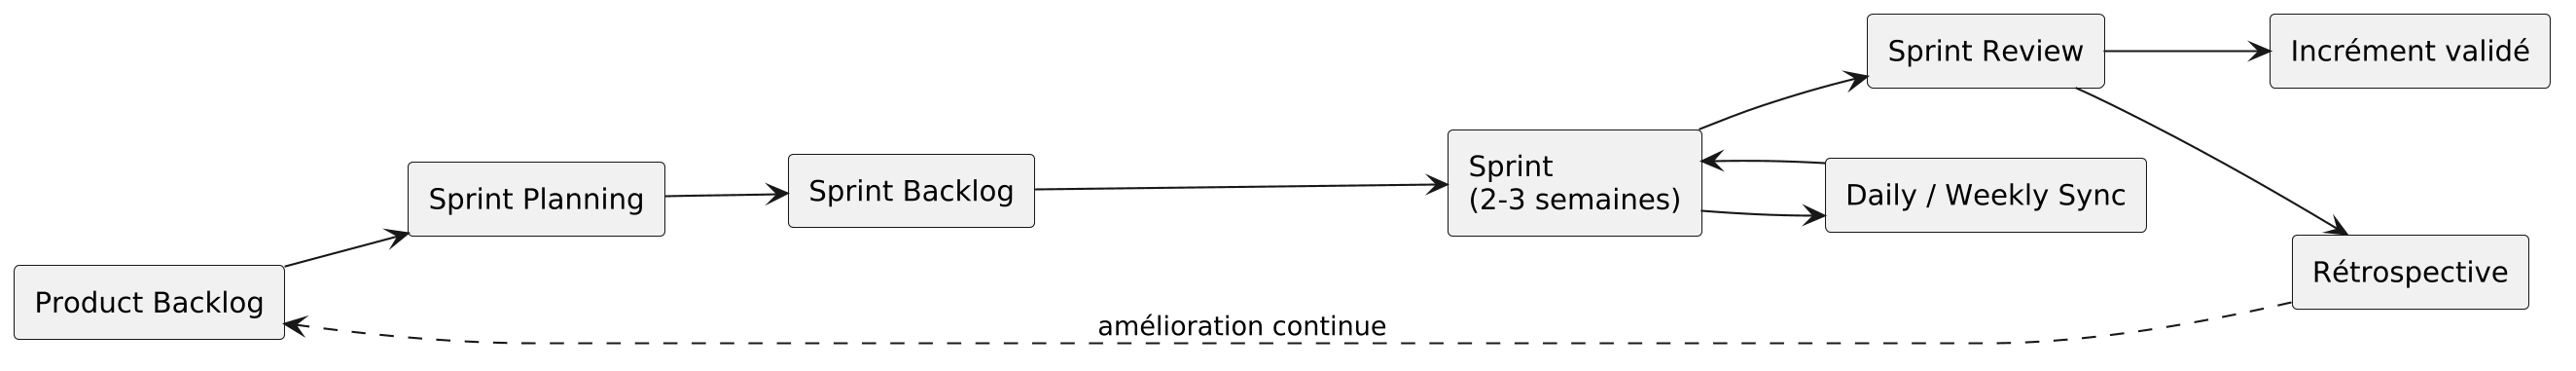
\includegraphics[width=0.88\textwidth,height=0.35\textheight,keepaspectratio]{img/fig_1_1_scrum.png}
    \caption{Processus M\'ethodologique Scrum Appliqu\'e au Projet CyberSec-ASM}
    \label{fig:scrum_process}
\end{figure}

\subsection{Product Backlog Global}
\par Le \textit{Product Backlog} constitue le r\'epertoire central de l'ensemble des exigences fonctionnelles et techniques du projet. Chaque exigence est formul\'ee sous la forme d'une \textit{User Story} (US) selon le formalisme standard : \textit{\og En tant que [Acteur], je veux [Action] afin de [B\'en\'efice] \fg{}}. Le tableau~\ref{tab:product_backlog} pr\'esente la liste ordonnanc\'ee des 30 User Stories prioritaires r\'eparties sur les six sprints.

\begin{table}[H]
\centering
\caption{Product Backlog Global du Projet CyberSec-ASM (30 User Stories)}
\label{tab:product_backlog}
\resizebox{\textwidth}{!}{%
\begin{tabular}{|c|L|L|c|c|c|}
\hline
\textbf{ID} & \textbf{Acteur} & \textbf{User Story (Description)} & \textbf{Priorit\'e} & \textbf{Est. (j)} & \textbf{Sprint} \\
\hline
US01 & Analyste / Admin & S'authentifier de mani\`ere s\'ecuris\'ee avec gestion des sessions JWT & Must Have & 2 & Sprint 1 \\
\hline
US02 & Administrateur & G\'erer les utilisateurs, assigner les r\^oles RBAC et les quotas & Must Have & 3 & Sprint 1 \\
\hline
US03 & Analyste & Cr\'eer un projet d'audit et configurer le p\'erim\`etre des cibles & Must Have & 3 & Sprint 1 \\
\hline
US04 & Analyste & T\'el\'everser et valider le document de preuve d'autorisation (PoA) & Must Have & 2 & Sprint 1 \\
\hline
US05 & Auditeur & V\'erifier la validit\'e juridique et l'historique des mandats PoA & Should Have & 2 & Sprint 1 \\
\hline
US06 & Analyste & Lancer un scan de reconnaissance (Nmap, Nuclei, Gobuster, etc.) & Must Have & 4 & Sprint 2 \\
\hline
US07 & Analyste & Choisir le profil d'intensit\'e de scan (Silent, Balanced, Aggressive) & Must Have & 2 & Sprint 2 \\
\hline
US08 & Analyste & Normaliser automatiquement les sorties brutes en format structur\'e JSON & Must Have & 4 & Sprint 2 \\
\hline
US09 & Analyste & Suivre l'\'etat d'avancement d'un scan en temps r\'eel via Redis Streams & Must Have & 3 & Sprint 2 \\
\hline
US10 & Analyste & Consulter les journaux bruts (\textit{raw logs}) avec citations de lignes & Should Have & 2 & Sprint 2 \\
\hline
US11 & Analyste & Ex\'ecuter des tests d'injection (SQLi, XSS, Command Injection) & Must Have & 4 & Sprint 3 \\
\hline
US12 & Analyste & D\'eployer un conteneur sandbox vuln\'erable isol\'e (DVWA, bWAPP) & Must Have & 4 & Sprint 3 \\
\hline
US13 & Analyste & D\'etruire et r\'einitialiser l'environnement de bac \`a sable & Must Have & 2 & Sprint 3 \\
\hline
US14 & Analyste & Tester la pr\'esence et le comportement d'un WAF externe & Should Have & 3 & Sprint 3 \\
\hline
US15 & Administrateur & Isoler le socket Docker via socket-proxy pour prot\'eger l'h\^ote & Must Have & 2 & Sprint 3 \\
\hline
US16 & Analyste & Solliciter l'IA locale pour analyser les constats de vuln\'erabilit\'e & Must Have & 4 & Sprint 4 \\
\hline
US17 & Analyste & G\'en\'erer des scripts de rem\'ediation durcis (Bash, Ansible, Dockerfile) & Must Have & 4 & Sprint 4 \\
\hline
US18 & Analyste & Valider le respect du sch\'ema Pydantic strict pour \'eviter les hallucinations & Must Have & 3 & Sprint 4 \\
\hline
US19 & Analyste & Appliquer et t\'el\'echarger les correctifs de s\'ecurit\'e propos\'es & Should Have & 2 & Sprint 4 \\
\hline
US20 & Analyste & Consulter la synth\`ese manag\'eriale et l'impact m\'etier g\'en\'er\'es par l'IA & Should Have & 2 & Sprint 4 \\
\hline
US21 & Analyste & Visualiser la topologie des actifs sous forme de graphe relationnel & Must Have & 4 & Sprint 5 \\
\hline
US22 & Analyste & Calculer le rayon d'impact (\textit{blast radius}) par l'algorithme BFS & Must Have & 3 & Sprint 5 \\
\hline
US23 & Analyste & Collecter des renseignements passifs OSINT (DNS, WHOIS, SSL) & Must Have & 3 & Sprint 5 \\
\hline
US24 & Client & Consulter la vue synth\'etique du tableau de bord restreinte \`a son scope & Must Have & 2 & Sprint 5 \\
\hline
US25 & Client / Analyste & Poser des questions de s\'ecurit\'e au Chatbot conversationnel IA & Should Have & 3 & Sprint 5 \\
\hline
US26 & Analyste / Client & G\'en\'erer et exporter les rapports d'expertise (PDF sign\'e, HTML, JSON) & Must Have & 4 & Sprint 6 \\
\hline
US27 & Client & Recevoir et acquitter les alertes de s\'ecurit\'e critiques & Must Have & 2 & Sprint 6 \\
\hline
US28 & Auditeur / Admin & Consulter le journal d'audit immuable (\textit{Audit Logs}) infalsifiable & Must Have & 3 & Sprint 6 \\
\hline
US29 & Auditeur / Admin & Superviser l'\'etat de sant\'e et la disponibilit\'e des microservices & Must Have & 2 & Sprint 6 \\
\hline
US30 & DevSecOps & Ex\'ecuter le pipeline CI/CD automatis\'e avec portes de s\'ecurit\'e & Must Have & 4 & Sprint 6 \\
\hline
\end{tabular}}%
\end{table}

\subsection{Sprint Backlogs D\'etaill\'es}
\par Afin de garantir une ex\'ecution m\'ethodique, les User Stories ont \'et\'e ventil\'ees en six \textit{Sprint Backlogs}. Chaque sprint comporte des objectifs pr\'ecis, des crit\`eres de validation et une charge estim\'ee en jours-homme.

\begin{table}[H]
\centering
\caption{D\'ecomposition D\'etaill\'ee des Sprint Backlogs (Sprints 1 \`a 6)}
\label{tab:sprint_backlogs_detail}
\resizebox{\textwidth}{!}{%
\begin{tabular}{|c|c|L|c|c|L|}
\hline
\textbf{Sprint} & \textbf{US ID} & \textbf{Intitul\'e de la T\^ache / User Story} & \textbf{Priorit\'e} & \textbf{Est. (j)} & \textbf{Crit\`ere d'Acceptation (DoD)} \\
\hline
\multirow{5}{*}{\textbf{Sprint 1}} & US01 & Authentification JWT et contr\^ole des sessions & Must & 2 & Token valide \'emis, expiration contr\^ol\'ee \\
\cline{2-6}
 & US02 & Gestion des r\^oles RBAC (Admin, Analyst, Auditor, Client) & Must & 3 & Middleware de filtrage par r\^ole actif \\
\cline{2-6}
 & US03 & Cr\'eation de projet et saisie du p\'erim\`etre des cibles & Must & 3 & Enregistrement en base PostgreSQL valid\'e \\
\cline{2-6}
 & US04 & T\'el\'eversement et validation du mandat PoA obligatoire & Must & 2 & V\'erification de signature et hachage SHA-256 \\
\cline{2-6}
 & US05 & Contr\^ole juridique des preuves d'autorisation & Should & 2 & Blocage logiciel si PoA absent ou expir\'e \\
\hline
\multirow{5}{*}{\textbf{Sprint 2}} & US06 & Int\'egration du moteur d'orchestration des scanners & Must & 4 & Ex\'ecution asynchrone de Nmap, Nuclei, etc. \\
\cline{2-6}
 & US07 & Gestion des profils de scan et param\'etrage du jitter & Must & 2 & Profils Silent, Balanced, Aggressive op\'erationnels \\
\cline{2-6}
 & US08 & Pipeline de normalisation des r\'esultats \texttt{ResultParser} & Must & 4 & Sorties JSON unifi\'ees avec s\'ev\'erit\'e et CVE \\
\cline{2-6}
 & US09 & T\'el\'em\'etrie temps r\'eel et suivi de progression Redis Streams & Must & 3 & \'Ev\'enements publi\'es et consomm\'es sans perte \\
\cline{2-6}
 & US10 & Visualisation des logs bruts et tra\c{c}abilit\'e des lignes & Should & 2 & Lignes de preuves surlign\'ees dans l'IHM \\
\hline
\multirow{5}{*}{\textbf{Sprint 3}} & US11 & Module d'audit d'injections et vuln\'erabilit\'es applicatives & Must & 4 & D\'etection confirm\'ee de failles OWASP Top 10 \\
\cline{2-6}
 & US12 & D\'eploiement dynamique de conteneurs sandbox isol\'es & Must & 4 & Instanciation DVWA/bWAPP en r\'eseau isol\'e \\
\cline{2-6}
 & US13 & Cycle de vie et destruction automatique des sandboxes & Must & 2 & Nettoyage complet des ressources apr\`es test \\
\cline{2-6}
 & US14 & D\'etection et \'evaluation de contournement WAF & Should & 3 & Rapports d'analyse WAF d\'etaill\'es \\
\cline{2-6}
 & US15 & Durcissement de l'acc\`es Docker via \texttt{socket-proxy} & Must & 2 & Interdiction des privil\`eges root sur l'h\^ote \\
\hline
\multirow{5}{*}{\textbf{Sprint 4}} & US16 & Int\'egration du serveur d'inf\'erence local Ollama & Must & 4 & Mod\`ele \texttt{qwen2.5-coder:7b} op\'erationnel \\
\cline{2-6}
 & US17 & G\'en\'eration automatis\'ee de scripts Remediation-as-Code & Must & 4 & Scripts Bash, Ansible et Dockerfile syntaxiques \\
\cline{2-6}
 & US18 & Validation stricte du format JSON via sch\'ema Pydantic & Must & 3 & 0\% d'hallucination de format en sortie \\
\cline{2-6}
 & US19 & T\'el\'echargement s\'ecuris\'e des correctifs de s\'ecurit\'e & Should & 2 & Fichiers de correction g\'en\'er\'es et sign\'es \\
\cline{2-6}
 & US20 & G\'en\'eration de synth\`eses d'impact pour d\'ecideurs & Should & 2 & R\'esum\'e manag\'erial clair et actionnable \\
\hline
\multirow{5}{*}{\textbf{Sprint 5}} & US21 & Mod\'elisation et affichage du Graphe de Connaissances & Must & 4 & Rendu interactif via Cytoscape.js \\
\cline{2-6}
 & US22 & Impl\'ementation du calcul de Blast Radius (BFS NetworkX) & Must & 3 & Propagation d'impact calcul\'ee en $<75$~ms \\
\cline{2-6}
 & US23 & Renseignement passif OSINT (DNS, WHOIS, Certificats) & Must & 3 & Donn\'ees agr\'eg\'ees sans envoi de paquets actifs \\
\cline{2-6}
 & US24 & Vue IHM restreinte pour le profil Client & Must & 2 & Dashboard filtr\'e sur les actifs autoris\'es \\
\cline{2-6}
 & US25 & Co-pilote conversationnel IA d'assistance & Should & 3 & R\'eponses contextuelles bas\'ees sur l'audit \\
\hline
\multirow{5}{*}{\textbf{Sprint 6}} & US26 & Moteur de g\'en\'eration et export de rapports d'expertise & Must & 4 & Rapports PDF, HTML et JSON t\'el\'echargeables \\
\cline{2-6}
 & US27 & Centre de notification et d'acquittement d'alertes & Must & 2 & Alertes par e-mail et interface web \\
\cline{2-6}
 & US28 & Journalisation immuable d'audit (\textit{Audit Logs}) & Must & 3 & \'Ev\'enements infalsifiables horodat\'es \\
\cline{2-6}
 & US29 & Surveillance de l'\'etat de sant\'e du syst\`eme (\textit{Health}) & Must & 2 & M\'etriques CPU, RAM, conteneurs affich\'ees \\
\cline{2-6}
 & US30 & Int\'egration du pipeline DevSecOps CI/CD sous GitHub & Must & 4 & 8 portes de s\'ecurit\'e bloquantes valid\'ees \\
\hline
\end{tabular}}%
\end{table}

\section*{Conclusion}
\par Ce premier chapitre a permis d'exposer le cadre g\'en\'eral du projet, en d\'emontrant par une analyse comparative approfondie les lacunes des outils existants et l'int\'er\^et d'une approche unifi\'ee semi-agentique. Nous avons d\'efini la probl\'ematique, les objectifs, le p\'erim\`etre et la m\'ethodologie de conduite Agile Scrum. Le chapitre suivant d\'eveloppe l'\'etat de l'art scientifique et l'\'etude comparative des technologies de r\'ef\'erence.
